\documentclass{article}
\usepackage[utf8]{inputenc}
\usepackage[spanish]{babel}
\usepackage{listings}
\usepackage{graphicx}
\graphicspath{ {images/} }
\usepackage{cite}

\begin{document}

\begin{titlepage}
    \begin{center}
        \vspace*{1cm}
            
        \Huge
        \textbf{Implementación de la solucion}
            
        \vspace{0.5cm}
        \LARGE
        
            
        \vspace{1.5cm}
            
        \textbf{Juan Camilo Mazo Castro}\\
        \textbf{Santiago Pereira Ramirez}
            
        \vfill
            
        \vspace{0.8cm}
            
        \Large
        Despartamento de Ingeniería Electrónica y Telecomunicaciones\\
        Universidad de Antioquia\\
        Medellín\\
        Septiembre de 2021
            
    \end{center}
\end{titlepage}

\tableofcontents
\newpage
\section{Clases Implementadas}\label{intro}
Para el desarrollo del parcial se creo una clase llamada imageresized al cual tiene atributos y metodos privados y metodos publicos los cuales proporcionan la funciones para el muestreo de la imagen insertada en el programa. Esta no tiene metodos sobrecargados o el constructor sobrecargado y utiliza algunas librerias como lo son string y fstream para el manejo de datos y llevarlos hacia un documento.txt, o tambien QImage para la extraccion de datos de la imagen ingresada.


\section{Esquema de la clase implementada }\label{contenido}

En la Figura 1 se podra ver la estructura de la clase implementada en el entorno de desarrollo Qrcreator:

\begin{figure}[h]
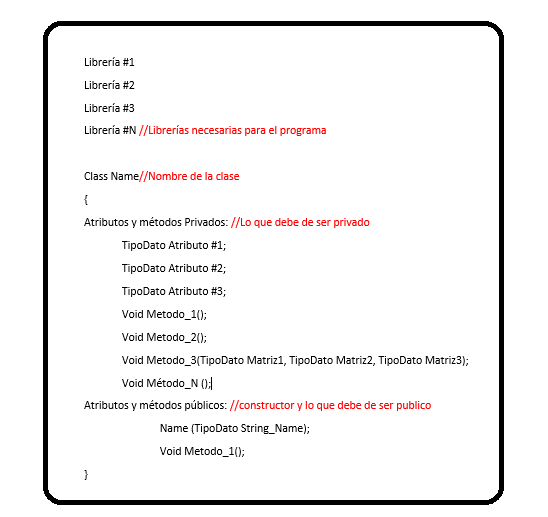
\includegraphics[width=10 cm]{Estructura_clase.PNG}
\centering
\caption{Estructura clase}
\label{fig:Estructura_clase}
\end{figure}


\section{Modulacion}\label{contenido}

En la figura 2 se podra ver la modulacion de la clase Imageresized:

\begin{figure}[h]
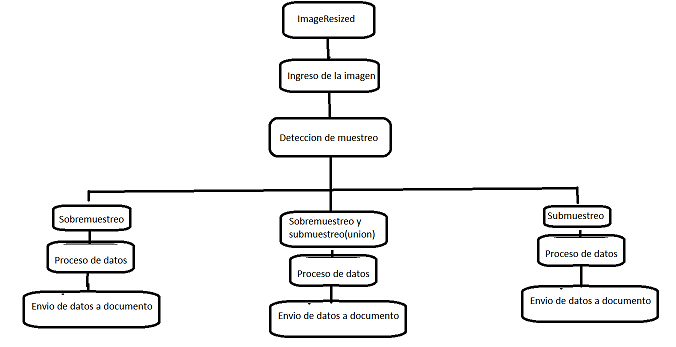
\includegraphics[width=13 cm]{Esquema.PNG}
\centering
\caption{Esquema de la clase}
\label{fig:Esquema}
\end{figure}

\section{Estructura del circuito}\label{contenido}

Para la construccion del circuito se utilizaron elementos como una placa electronica arduino, un suministro de energia y 16 tiras de leds neopixel. Primero por medio del pin 2 del arduino lo conectamos a la entrada de la primera tira de neopixel, despues atravez del GND(tierra) del arduino lo conectamos en la tierra del suministro de energia y este a su vez a la tierra de la primera tirilla de neopixel. Respecto a la potencia se empalmo directamente del suministro de energia a la potencia de la primera tira de neopixel.\\

Ahora por medio de la salida de la primera tirilla de neopixel se conectara a la entrada de la siguiente tirilla de neopixel, al igual que la potencia y la tierra repitiendo este proceso hasta terminar con las tiras.\\

A continuacion se podra ver un pequeño ejemplo en la figura 3.\\


\begin{figure}[h]
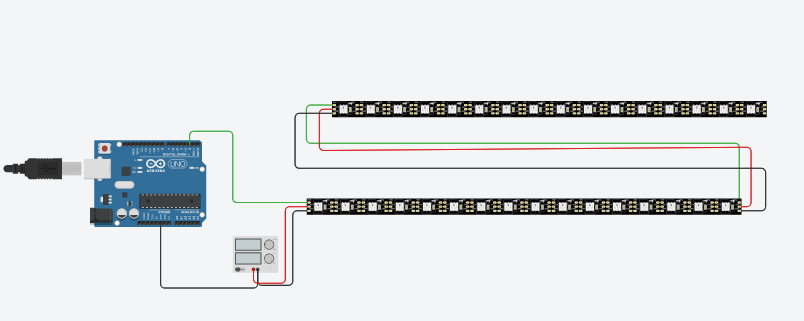
\includegraphics[width=8 cm]{Ejemplo_circuito.PNG}
\centering
\caption{Ejemplo estructura circuito}
\label{fig:Ejemplo_circuito}
\end{figure}


\section{Problemas presentados}\label{contenido}

Durante el desarrollo del programa y montaje del circuito se presentaron alguno problemas como puede ser:\\

--Al utilizar tres arreglos para almacenar los datos en tinkercad la ejecucion y en general para mostrar la bandera se tardaba bastante tiempo, para solucionarlo se debio de utilizar un arreglo tridimensional y (for)  anidados para mandar los datos.\\

--Al ejecutar el programa en tinkercad seguia tardando mucho, esto ya que era problema del propio computador y conexion a internet de un participante, por el contrario el del otro compañero se ejecutaba rapido y eficaz.Esto ocaciono que algunas veces se cambiara el Hardware, pero al final no hubo una necesidad de cambiar la estructura inicial del mismo.\\

--En el programa se trabajo especialmente con arreglos, esto ocasiono que al ingresar imagenes muy grandes se llenara el stack, para dar solucion a esto se recurrio a mamoria dinamica.\\

--Se tuvieron algunos inconvenientes con el Github y los repositorios, ya que se clono mal en un caso y ademas el enlace avaces tardaba mucho entre el repositorio remoto y local.\\

\end{document}
